\subsection{General Strategy}
The majority of problems in this chapter is focused on using Coulomb's Law. Because force is a vector, it can sometimes be hard to keep track of all the different directions. First, calculate the magnitude of each individual force, then break the force into components. Then, superimpose all the forces by summing them up.\footnote{Remember, you can't sum magnitudes, but you can sum vectors} If it is needed, convert back to magnitude only at the end.

\subsection{Analog to Gravitation}
Hopefully, you can already see the similarities between electrostatics and gravitation. If not, we will point it out below. The force between two charges is almost exactly equivalent to the force between two masses.
\\\\
Coulomb's Law: $F=\frac{1}{4\pi\epsilon_0}\frac{Q_1Q_2}{R^2}$
\\
Newton's Law of Gravitation: $F=G\frac{M_1M_2}{R^2}$
\\\\
Notice how the gravitational constant is a direct analog to coulomb's constant and how mass is a direct analog to charge. Even the principle of superposition holds true for both gravitation and electrostatics. Furthermore, the electric field $E$ can also be seen as a direct analog to gravitational acceleration $g=G\frac{M}{R^2}$
\\\\
\emph{Unlike} gravitation however, the force does not always act towards one direction. Masses can only attract one another, but charges can attract as well as repel. When two charges repel, their force is positive.
\\\\
More similarities will be pointed out in the chapters to come.

\subsection{Electric Field Lines}
The electric field is a vector field, meaning it assigns a vector (basically an arrow) to every point in space, such as in the figure below. The red lines represent the electric field at that point and flow from positive charges to negative charges: \footnote{The contour lines are equipotential lines, discussed in the next section about Energy Conservation.}

\begin{center}
% \begin{tikzpicture}
% \begin{axis}[axis equal image,domain=-4.05:4.05,,xmin=-4,xmax=4,ymin=-4,ymax=4,samples=40,view={0}{90}]

%   \addplot3[contour gnuplot={number=50,labels=false, draw color=blue},thick,]
%               {abs(((1)/sqrt((x-2)^2+y^2) - (1)/sqrt((x+2)^2+y^2)))<4 ? ((1)/sqrt((x-2)^2+y^2) - (1)/sqrt((x+2)^2+y^2)) : NaN };
% %set to 18
%   \addplot3[contour gnuplot={number=18,labels=false, draw color=red},
%              thick,
%             ]
%              {abs(((x-2)/sqrt((x-2)^2+y^2) - (x+2)/sqrt((x+2)^2+y^2)))<10 ? ((x-2)/sqrt((x-2)^2+y^2) - (x+2)/sqrt((x+2)^2+y^2)) : NaN };
% \end{axis}
% \end{tikzpicture}
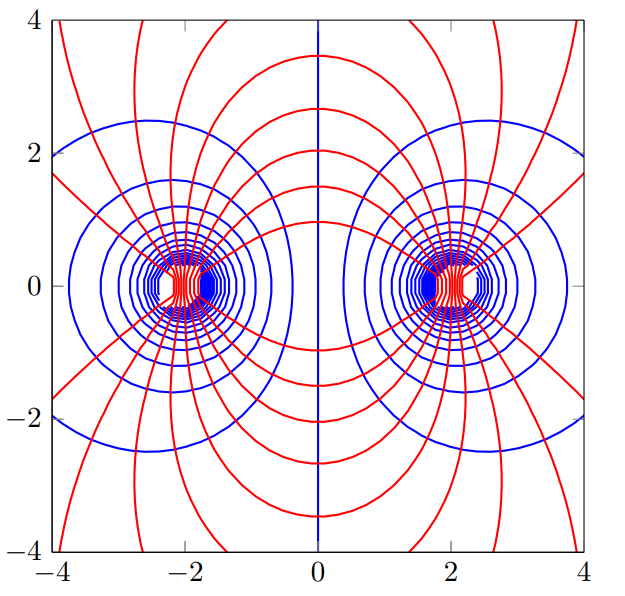
\includegraphics{Figures/Figure21}
\end{center}

Important properties of electric field lines which can be used in problem solving are listed below:
\begin{enumerate}
    \item The lines begin and end only on charges. As a result, the lines are spaced such that they are bunched more closely together in areas of strong field and spaced more widely apart in areas of weak field.
    \item Because the electric field can have only one unique direction at any location in space, the lines may never intersect in a location where the direction of the electric field is well defined
    \item The lines represent the direction of the force. In general, the lines do not represent the \emph{trajectory} of a particle moving only under the influence of the electric field.\footnote{Why? From mechanics, we know that for a particle to move along a curved path, it must have a radial acceleration. If a particle were moving along a curved electric field line, because the force is parallel to the field line, there would be no force providing the radial acceleration - that would be impossible!}
\end{enumerate}

\newpage
\subsection{Energy Conservation Problems}
Because potential, or voltage: $V$ is a measure of potential energy \emph{per} charge, it is easily used to calclate the potential energy of a specified charge and thus is useful in problems involving energy conservation.
\\\\
Potential is a \emph{scaler} meaning we can assign a single value to every single point on the x,y plane. Because of this, we can represent potential in two dimensions using \emph{equipotential lines}, which are lines of constant potential in the two-dimensional plane. By providing a series of equipotential lines at equally spaced intervals (i.e., plotting when potential is 1V, 2V, 3V, and so on) a contour plot can be created similar to topographical maps that display different altitudes in different colors. Here are important properties of potential lines when problem solving
\begin{enumerate}
    \item Because potential is constant along an equipotential line, no force or work is required to move a charge along a given equipotentia line
    \item Recall $W=Fdcos(\theta)$ Because no work is required, this means $\theta$ must be $90^\circ$ meaning \emph{the equipotential lines is perpendicular to the electric field}
    \item When the electric field is stronger, the potential lines are bunched closer together. If you know calculus, you can use (2.5) to prove this.
\end{enumerate}

% \begin{tikzpicture}
% \begin{axis}[
%     view={0}{90},
%     clip = false,
%     xmin = -4,
%     xmax = 4,
%     ymin = -2.3,
%     ymax = 2.3,
%     point meta min = -4,
%     point meta max = 3,
%     y axis line style={draw opacity=0},
%     x axis line style={draw opacity=0},
%     xtick=\empty,
%     ytick=\empty,
%     unit vector ratio=1 1 1,
%     width=\linewidth,
%     colormap name=viridis
%     ]
% \addplot+[
%     no markers,
%     raw gnuplot,
%     contour prepared,
%     contour/labels=false
%     ] gnuplot {set samples 50, 50;
%             set isosamples 55, 55;
%             set contour base;
%             set cntrparam levels incremental -4,0.22,4;
%             set style data lines;
%             splot [-4:4] [-2.3:2.3] (-2/sqrt((x+2)**2+y**2)-1/sqrt((x-2)**2+y**2));
%             };
% \end{axis}
% \end{tikzpicture}
\begin{center}
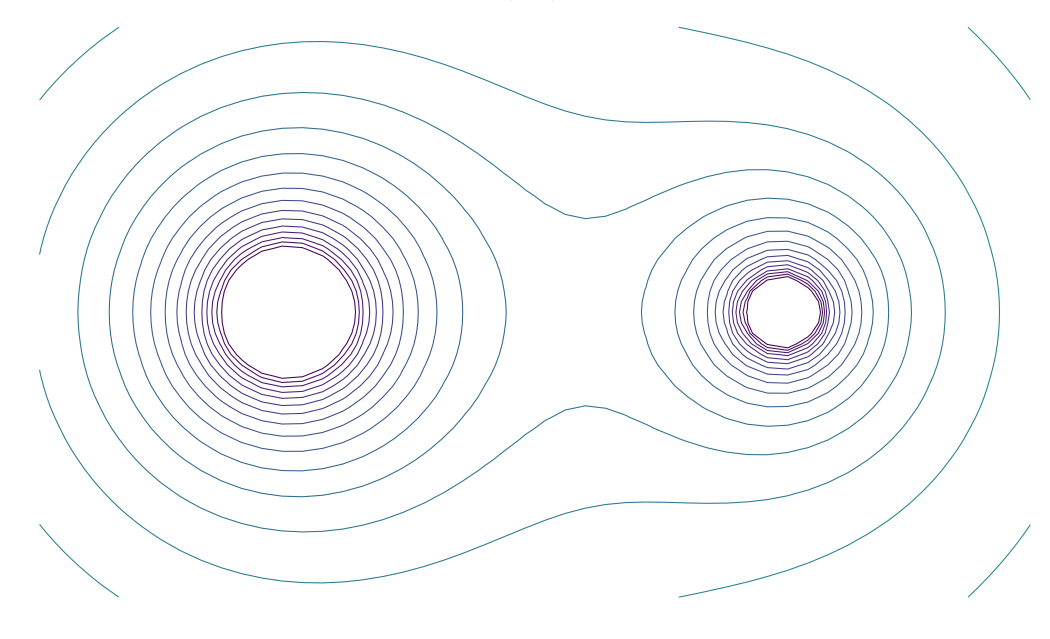
\includegraphics[scale=0.7]{Figures/Figure22}
\end{center}
\\\\
Here is a sample contour plot of equipotential lines. Based solely on this diagram and using the tricks provided, can you:
\begin{enumerate}
    \item Identify the source of the charges?
    \item Identify where the electric field is weakest?
    \item Draw the electric field lines?
\end{enumerate}